% Plantilla simple para tareas de la Licenciatura en Física
% Fer Flores - Universidad de Guadalajara - Noviembre 2023

%%%%%%%%%%%%%%%%%%%%%%%%%%%%%%%%%%%%%%%%%%-PREÁMBULO-%%%%%%%%%%%%%%%%%%%%%%%%%%%%%%%%%%%%%%%%%%

% Paqueterías

\documentclass{assignment}
\usepackage[pdftex]{graphicx} % FIGURAS
\usepackage{xcolor}
\definecolor{LightGray}{gray}{0.95}
\usepackage{fancyvrb, minted} % CÓDIGO
\usepackage[letterpaper, margin = 2.5cm]{geometry} % TAMAÑO DE PÁGINA Y MÁRGENES
\usepackage[T1]{fontenc} % Importante para acentos automáticos y símbolos de escritura
\usepackage{amsmath, amsfonts, amssymb} % Ecuaciones, caracteres y símbolos especiales
\usepackage{hyperref, url}  % Links y Hyperlinks en el documento
\usepackage{fancyhdr}

%-----------------------------------------ETIQUETAS--------------------------------------------

\student{Name Username, student-id} 
\semester{2023-2024}
\date{\today} 

\courselabel{Automatic Verification of Intelligent Systems}          % CLAVE Y MATERIA
\exercisesheet{}{\today}

\school{Computer Science}
\university{Università degli Studi di Roma "La Sapienza"}         % LA PODEROSÍSIMA

%%%%%%%%%%%%%%%%%%%%%%%%%%%%%%%%%%%%%%%%%%-DOCUMENTO-%%%%%%%%%%%%%%%%%%%%%%%%%%%%%%%%%%%%%%%%%%%%

\begin{document}

%-----------------------------------------------------------------------------------------------
%\begin{problem}

\section{Stochastic Processes}

\subsection{Stationary processes}
\noindent Yes, it is \emph{strictly stationary} because at every time step $t$ the sample is drawn from the very same distribution which is $X_t$ with mean $0$ and variance $1$.

\subsection{Mean stationary processes}
\noindent The process is \emph{mean stationary}.
$$ \mathbb{E}[X_t] = \mathbb{E}[Acos\left(\omega t + \theta\right)] = \underbrace{\mathbb{E}[A]}_0\mathbb{E}[cos\left(\omega t + \theta\right)] = 0$$


\subsection{Covariance stationary processes}
\noindent The process is \emph{covariance stationary} because it depends only on the \textbf{time difference} $k$.
$$ \mathbb{E}[X_t]  = \mathbb{E}[Asin(\omega t + \theta)] = \underbrace{\mathbb{E}[A]}_0\mathbb{E}[sin(\omega t + \theta )] = 0$$
$$ \mathbb{E}[X_t X_{t+k}] = \mathbb{E}[A^2sin(\omega t + \theta)sin\left( \omega \left(t + k \right) + \theta \right)] $$
$$= \mathbb{E}[A^2] \mathbb{E}\left[ \frac{1}{2}(cos(\omega k) - cos(\omega (2t+k) + 2\theta)) \right]$$
$$= \frac{1}{2} cos(\omega k) - \frac{1}{2}\int_{-\pi}^{\pi}cos\left( \omega(2t+k)+2\theta \right)\frac{1}{2\pi}d\theta$$
$$= \frac{1}{2}cos(\omega k)-\frac{1}{8\pi}\left[ sin(\omega (2t+k)+2\theta) \right]_{-\pi}^\pi$$
$$ = \frac{1}{2}cos(\omega k)$$

\subsection{Moments from samples}
\subsubsection{Sample mean}
The sample mean is:
$$\Bar{X} = \frac{1}{n}\sum_{i=1}^{n}X_i = -0.152$$

\subsubsection{Sample covariance}
\noindent The sample covariance with lag $0$ is
$$\Hat{\gamma}_0 = \frac{1}{n}\sum_{i=1}^{n}(X_t-\Bar{X})(X_t-\Bar{X}) = 0.286$$

\subsubsection{Sample autocorrelation}
\noindent The autocorrelation at lag $k=1$
$$\Hat{\rho}_1 = \frac{\Hat{\gamma_1}}{\Hat{\gamma_0}} = 0.0046$$
Where $\Hat{\gamma_1 = 0.0013}$

\subsection{Difference equations}
\noindent The roots are:
$$R_1 = (0.5 - 0.866i)$$
$$R_2 = (0.5 + 0.866i)$$

We should then find:
$$\alpha = 1$$
$$\phi = 1.0472 = \frac{\pi}{3}$$

So the closed form solution is:
$$ Z_t = b_1\alpha^t cos(\phi t) + b_2\alpha^t sin(\phi t) = b_1cos(\frac{\pi}{3}t) + b_2sin(\frac{\pi}{3}t)$$

\subsection{AR processes variance}
\noindent The variance is: 
$$ \gamma_0 = \frac{\sigma_a^2}{1-\phi_1^2} = 1.041 $$
Where $\phi_1 = 0.2$ 

\subsection{AR process covariance}
\noindent The covariance with lag $k=1$ is:
$$\gamma_1 = \phi_1\gamma_0 = 1.372$$
Where $\phi_1 = 0.7$ 

\subsection{AR process autocorrelation}
\noindent The autocorrelation with lag $k=1$ is:
$$\rho_1 = \frac{\gamma_1}{\gamma_0} = 0.3 $$
With $\phi_1 = 0.3$

\subsection{MA processes variance}
\noindent The variance is: 
$$ \gamma_0 = (1+\theta_1^2)\sigma_a^2 = 1.04$$
Where $\theta_1 = -0.2$ 

\subsection{MA process covariance}
\noindent The covariance with lag $k=1$ is: 
$$\gamma_1 = \theta_1\sigma_a^2 = -0.7$$
Where $\theta_1 = -0.7$ 

\subsection{MA process autocorrelation}
\noindent The autocorrelation with lag $k=1$ is:
$$\rho_1 = \frac{\gamma_1}{\gamma_0} = -0.275 $$
With $\theta_1 = -0.3$


\subsection{ARIMA processes variance}
\noindent The variance is: 
$$ \gamma_0 = \frac{1+\theta_1^2+2\phi_1\theta_1}{1-\phi_1^2}\sigma_a^2 = 1.01$$
Where $\theta_1 = -0.1$ and $\phi_1 = 0.2$

\subsection{ARIMA process covariance}
\noindent The covariance with lag $k=1$ is: 
$$\gamma_1 = \phi_1\gamma_0 + \theta_1\sigma_a^2 = 0.102$$
Where $\theta_1 = -0.1$ and $\phi_1 = 0.2$

\subsection{ARIMA process autocorrelation}
\noindent The autocorrelation with lag $k=1$ is:
$$\rho_1 = \frac{\gamma_1}{\gamma_0} = 0.101 $$


\subsection{Model identification 1}
\noindent The most suited model for the process is an \textbf{AR(2)} model with $\phi_1 > 0$ and $\phi_2 < 0 $.
\begin{figure}[H]
    \centering
    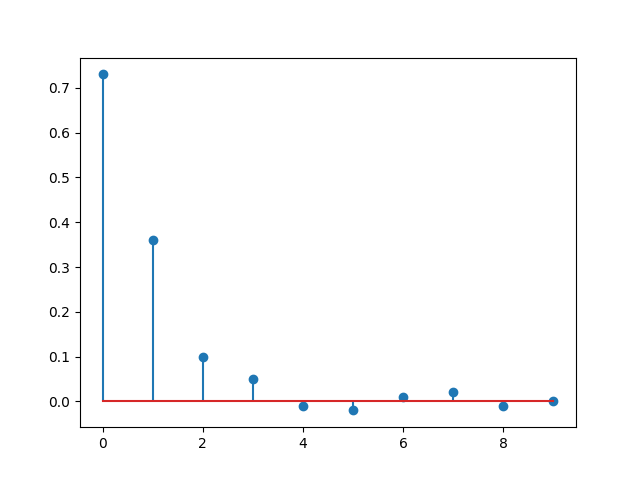
\includegraphics[width=0.5\linewidth]{Figuras/model-1.png}
    \caption{$\rho_k$ of the model.}
    \label{fig:enter-label}
\end{figure}


\subsection{Model identification 2}
\noindent The most suited model for the process is an \textbf{MA(2)} model with $\theta_1 < 0$ and $\theta_2 < 0$.
\begin{figure}[H]
    \centering
    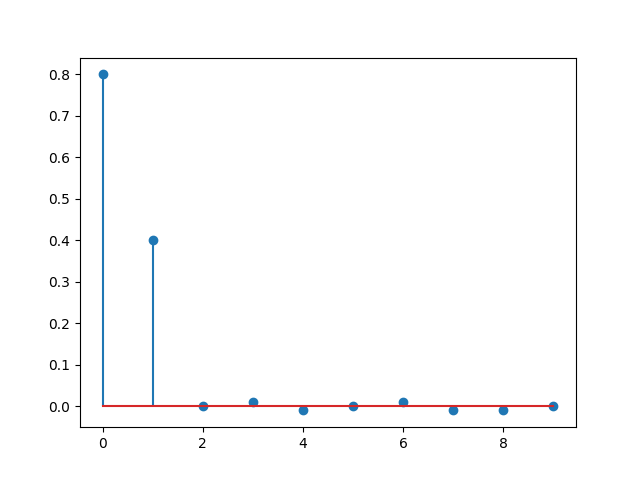
\includegraphics[width=0.5\linewidth]{Figuras/model-2.png}
    \caption{$\rho_k$ of the model.}
    \label{fig:enter-label}
\end{figure}


\section{Optimization}
\subsection{Constants} These are the constants of the problem
\begin{itemize}
    \item $n$: number of warehouses
    \item $m$: number of customers
    \item $f_i$: fixed minimum operating cost of warehouse
    \item $c_ij$: cost of production and shipment of one unit from warehouse $i$ to customer $j$
    \item $d_j$: demand of items required from customer $j$
\end{itemize}

\subsection{Variables} These are the variables that the optimizer will try to solve for
\begin{itemize}
    \item $\{x_{ij} \in \mathbb{N}\,|\,i \in [1,n], j \in [1,m]\} = \mathcal{X}$: amount of items to be made and shipped from warehouse $i$ to client $j$
    \item $\{y_i \in \{0,1\} \,|\,i \in [1,n] \} = \mathcal{Y}$: if the warehouse $i$ is open (1) or not (0)
\end{itemize}

\subsection{Objective}
This is the objective function that the optimizer will try to minimize
$$ argmin_{\mathcal{X},\mathcal{Y}} \sum_{i=1}^n \sum_{j=1}^m \left( x_{ij}c_{ij} + y_if_i \right) $$

\subsection{Customer Demands}
This constraint enforces that the customers' demands be satisfied
$$\sum_{i=1}^n x_{ij} \geq d_j \quad \forall j \in [1,m] $$

\subsection{No shipments from closed warehouses}
Let $M = \sum_{j=1}^m d_j$ then we have that the constraint that enforces shipments to be made only from open warehouses is
$$ x_{ij} \leq My_i \quad \forall i \in [1,n] \;\,\forall j \in [1,m] $$

\end{document}